\documentclass{article}

% Language setting
% Replace `english' with e.g. `spanish' to change the document language
\usepackage[french]{babel}
\usepackage[T1]{fontenc}

% Set page size and margins
% Replace `letterpaper' with`a4paper' for UK/EU standard size
\usepackage[letterpaper,top=0.5cm,bottom=0.5cm,left=2cm,right=2cm,marginparwidth=1.75cm]{geometry}

% Useful packages
\usepackage{amsmath}
\usepackage{graphicx}
\usepackage[colorlinks=true, allcolors=blue]{hyperref}
\usepackage{wrapfig}
\usepackage{enumitem}
\usepackage{subcaption}

\usepackage{tikz}
\usepackage[european, straightvoltages, RPvoltages, cute inductor]{circuitikz}  % RPvoltages definie la convention des dipoles (sens tension faux sinon)
\usetikzlibrary{babel}

\newcommand{\comment}[1]{}

% Colonnes
\newenvironment{col}[1]
{\begin{minipage}[t]{\dimexpr \textwidth * #1/100 - 0.03\textwidth}}{\end{minipage}\hspace{0.03\textwidth}}
\newenvironment{colf}[1]
{\begin{minipage}[t]{\dimexpr \textwidth * #1/100}}{\end{minipage}}
\newcommand{\twoCol}[3][50]{
    \begin{col}{#1}
        #2
    \end{col}
    \begin{colf}{\numexpr 100 - #1\relax}
        #3
    \end{colf}
}

\title{Filtres Eléctroniques Passifs}
\author{Raphaël Jamann}
\date{} % remove the date

\begin{document}
    \maketitle


    \section{Qu'est ce qu'un filtre}
    
    Un filtre est un quadripôle linéaire (constitué de dipôles linéaires R,L et C) qui \textbf{permet
    d'atténuer certaines fréquences} en régime sinusoïdal. 

    \bigskip
    Les filtres fonctionnent grâce à l'impédance complexe des dipôles R et C qui dépendent
    de la pulsation $\omega$ et donc de la fréquence $f=\frac{\omega}{2\pi}$. \\
    En effet, l'impédance d'un condensateur est $\underline{Z}_C=\dfrac{1}{j\omega C}$ . \\
    L'impédance d'une bobine L est $\underline{Z}_L=j\omega L$


    \section{Exemples de filtres passe haut}

    \twoCol{      
        \centering

        \subsection{High Pass RC Filter}

        \vspace{2mm}
        \begin{circuitikz}        
            % Circuit code
            \draw (0,0) to[short,o-o] ++ (4,0);
            \draw (0,2) to[C, l_=C, o-] ++ (3,0) coordinate(a);
            \draw (a) to[short, -o] ++ (1,0);
            \draw (a) to[R, name=R, *-*] ++(0,-2);
            \node at (R.center) {R};  % draw label "R" at the center of the resistance

            % Voltage labels
            \draw (0,2) to[open,v=V$_{\text{in}}$\;] ++(0,-2);
            \draw (4,2) to[open,v^=\hspace{1.5mm} V$_{\text{out}}$] ++(0,-2);
        \end{circuitikz}

        Sur ce montage, lorsque la fréquence est basse, l'impédance du condensateur est très
        grande donc la tension de sortie est plus faible que celle d'entrée. \\
        Lien de la \href{https://www.falstad.com/circuit/circuitjs.html?ctz=CQAgjCAMB0l3BWcBOaAOAbAdgCwCYsBmHMBMHZNQkBSGmuhAUwFowwAoANxAzxxB4EGXvxCE0AuhAyMo8mAg4B3UQIkCsCPOMlQOAJxBadQkSd1SGHAB7HkWcXhFosaJ8hACxANQA6AM4BAPYGAC4Alky2XlpOIsJIhHie3gL+AUwAdmEGAJfRqhZmIGhwgsL6RdqWpeUaVWoVCVgiJZAqTQ0IrbUddghoSGCEnmXU5DppIABiEQA2uUyBAA4AhkHLAQAWawCuYYEASgDCMTho7mDIdGjIw8jUAmAiAIKBsgASAF6BwVmrJgHQJcYIRAyBACOey28zWgTC2QCEX+gQAJlsQuEooEmAFDgE1mEwnksnsCtAOABjJolYqVKSweCQZCstnsjmpdAYNB4Xk4Igs5yXKBMiAdYLyZLyHAsq50GDirxSwTyHSEDhAA}{simulation}.
    }{
        \centering

        \subsection{High Pass RL Filter}
        
        \vspace{2mm}
        \begin{circuitikz}        
            % Circuit code
            \draw (0,0) to[short,o-o] ++ (4,0);  % draw the bottom wire
            \draw (0,2) to[R, name=R, o-] ++ (3,0) coordinate(a);  % draw the resistance
            \node at (R.center) {R};  % draw label "R" at the center of the resistance
            \draw (a) to[short,-o] ++ (1,0);  % draw wire to the right of R
            \draw (a) to[L, l_=L, *-*] ++(0,-2);  % draw the Capacitor

            % Voltage labels
            \draw (0,2) to[open,v_=V$_{\text{in}}$\;] ++(0,-2);
            \draw (4,2) to[open,v^=\hspace{1.5mm} V$_{\text{out}}$] ++(0,-2);
        \end{circuitikz}

        Sur ce montage, lorsque la fréquence est basse, l'impédance de la bobine est faible
        donc la tension de sortie est faible également.
        $$\underline{V}_{out}(t) = \underline{Z}_L \, \underline{i}(t) = \underline{Z}_L=j\omega L \, \underline{i}(t)$$
        Lien de la \href{https://www.falstad.com/circuit/circuitjs.html?ctz=CQAgjCAMB0l3BWcAmWDLMgZgBxmcgCxg4CcS6IFkVApgLRhgBQAbiIVsiMggGwcuHMAJoQ+NJDWnQEzAE6DuvAQgDsAlVB6RmAdyobhAzt2Kj9SnvxC5C1iwdPHbOe+aiX1mm3yIPPA28XP3cRTwAPW0gkMFIBNXxwUlIOcAEAQQAdAGcJAAkAL1yAewA7XIAHWgBXABdc1hKAS3lcgEca2lyAGwBDXLraMpzm8tyAE26cnJL5Oubp2hyGnL66uoBLsprN2mhmKOIccAR7BHJTtTT-ADFmnrr5acq+memACz76w54cGiwnFsagBhBMPHsADVcsMnntfnxCEhAfY1MgBIDrvZ-NCZnMFrRmD1DD5VEYPDJIBB6DBkFg1IRkGpEmpSAREoQYp4StoTjROaQTlJYLxtFhwBAxBAsMwgA}{simulation}.    
    }


    \section{Exemples de filtres passe bas}

    \twoCol{      
        \centering

        \subsection{Low Pass RC Filter}

        \vspace{2mm}
        \begin{circuitikz}        
            % Circuit code
            \draw (0,0) to[short,o-o] ++ (4,0);  % draw the bottom wire
            \draw (0,2) to[R, name=R, o-] ++ (3,0) coordinate(a);  % draw the resistance
            \node at (R.center) {R};  % draw label "R" at the center of the resistance
            \draw (a) to[short,-o] ++ (1,0);  % draw wire to the right of R
            \draw (a) to[C, l_=C, *-*] ++(0,-2);  % draw the Capacitor

            % Voltage labels
            \draw (0,2) to[open,v_=V$_{\text{in}}$\;] ++(0,-2);
            \draw (4,2) to[open,v^=\hspace{1.5mm} V$_{\text{out}}$] ++(0,-2);
        \end{circuitikz}

        Sur ce montage, lorsque la fréquence est haute, l'impédance du condensateur est basse
        donc la tension de sortie est basse également.
        $$\underline{V}_{out}(t) = \underline{Z}_C \, \underline{i}(t) = \dfrac{1}{j\omega C} \, \underline{i}(t)$$
        Lien de la \href{https://www.falstad.com/circuit/circuitjs.html?ctz=CQAgjCAMB0l3BWK0AckDMYwE4As3sA2SQgdgCYFsQFIaa6EBTAWiwCgA3EXdckSoR58eYIXQhh49OrOgJ2AJ2H9BNUkLV1ykdgHd1Q3GJWjx7AMaGBCIQg1meyeJAjloU9IQT40hNNhYpM6uUPqmaugouDbmBrz8xkJRMUlhBvaatiCE5DFa4ZmOuakmugAeIOiQSDhCpFjgBE4mAIIAOgDOYADWABIAXl0A9gB2XQAOTACuAC5dnMMAlopdAI7TTF0ANgCGXbNMo51LY10AJludncOKs0tXTJ3znbuzswCXo9MfTNDslWMKHAPhoKGCYHsTjyIAAYkttrNFFcJrtrlcAEZogECNBVXhVUh0dC4IwCGIANS6RyRvxxhFwSBJMQoyVwwXylK6NzuD3Ywyg4EFuEg2GBSBgkEogv46DCQA}{simulation}.    
    }{
        \centering

        \subsection{Low Pass RL Filter}

        \vspace{2mm}
        \begin{circuitikz}        
            % Circuit code
            \draw (0,0) to[short,o-o] ++ (4,0);
            \draw (0,2) to[L, l_=L, o-] ++ (3,0) coordinate(a);
            \draw (a) to[short, -o] ++ (1,0);
            \draw (a) to[R, name=R, *-*] ++(0,-2);
            \node at (R.center) {R};  % draw label "R" at the center of the resistance
    
            % Voltage labels
            \draw (0,2) to[open,v=V$_{\text{in}}$\;] ++(0,-2);
            \draw (4,2) to[open,v^=\hspace{1.5mm} V$_{\text{out}}$] ++(0,-2);
        \end{circuitikz}

        Sur ce montage, lorsque la fréquence est haute, l'impédance de la bobine est
        grande donc la tension de sortie est plus faible que celle d'entrée. \\
        Lien de la \href{https://www.falstad.com/circuit/circuitjs.html?ctz=CQAgjCAMB0l3BWc0BsBmSAOMB2HAWBATk0xXIgUhCSpoFMBaMMAKADcQUAmfEbhCi68QaTH2oQw8GlDkwErAO7C+YvjgTdR4qKwA2q-oJCbtAoZKixEkMGnyYsaFNkiuJrAE6mtxoWY6EuDwrAAepkQ4otxCmDiYMUQgfCIAagA6AM5ZAPZeAC4AlvThKZoxQoJIaNzJqXyZWfQAdgVeAJelKoEWIE7UfZDKvtrq-XBBeio8qSYIOEJDI7NTC0LjwxHEyfbJi4lg+NoNIABiRfrt9NkADgCGOTdZAEaPZY6HRNSYRHxgRDQKXAQgAgtkwABrAASAC9srkWnd6ABXArZdi5IpebIARxRz3092yBVaWSKiOyABNnnlCiVsvQsuisvcCgUOi0UV1oKxcnIINR8JASLIYILgdQgUCpaJWEA}{simulation}.

    }


    \comment{\section{Exemple de filtre passe bande}
    
    {\centering
    \begin{circuitikz}        
        % Circuit code
        \draw (0,0) to[short,o-o] ++ (4.5,0);
        \draw (0,2) to[short,o-] (0.5,2) to[L, l_=L] (2,2) to[C, l_=C] (3,2) -- (3.5,2) coordinate(a);
        \draw (a) to[short, -o] ++ (1,0);
        \draw (a) to[R, name=R, *-*] ++(0,-2);
        \node at (R.center) {R};  % draw label "R" at the center of the resistance

        % Voltage labels
        \draw (0,2) to[open,v=V$_{\text{in}}$\;] ++(0,-2);
        \draw (4.5,2) to[open,v^=\hspace{1.5mm} V$_{\text{out}}$] ++(0,-2);
    \end{circuitikz}

    Lien de la \href{https://www.falstad.com/circuit/circuitjs.html?ctz=CQAgjCAMB0l3BWcA2aAOMB2ALGXyEw1sESQFJzzKEBTAWjDACgA3EZAJmxE4WQ7cQAZmJRw4eFUozoCZgHdBPUT0wJOIsZGYAnEOs18BhrT0pgdADwMBOTCM4C0mNI9sgeQgGoAdAM7+APa6AC4AlrTMNtjqjgL8SMKcHl48fv60AHahugCXUUqmxiBocLz8UIoGGmal5apVSlxelQiYAiU6zUKN7QKN1uRoSGDCHmjCDniaaSAAYuEANrm0AQAOAIaBa-4ARptZACa7AEoAMgDC0Z5obmC2lLbI07bCniggAIIByJAAEgAvAK0UIBTYBMAAayBASCWQ2tAArmD-KwguFdAEAI5I3ZLCH+ULZfzheEBE4BYJhSIgong0KhPJZJEFaDMADGygqAmQdx5Hxg8EgtlFYvFEo89CFkEwwmE2GQtmwkGw3A6bwcMogOiWHH5JWKlVkkAg0tgZWw4wIhCVz04kyqQXEYAElBVtnush1gpEvHEmmEzCAA}{simulation}.
    }



    \section{Exemple de filtre coupe bande}
    
    \twoCol{
        \centering
        \begin{circuitikz}        
            % Circuit code
            \draw (0,0) to[short,o-o] ++ (4.5,0);
            \draw (0,2) to[short, o-] ++ (1,0) to[short] ++ (0,0.75) to[C, l_=C] ++ (1.5,0) to[short] ++ (0,-0.75) -- (3.5,2) coordinate(a);
            \draw (1,2) to[short] ++ (0,-0.75) to[L, l_=L] ++ (1.5,0) to[short] ++ (0,0.75);
            \draw (a) to[short, -o] ++ (1,0);
            \draw (a) to[R, name=R, *-*] ++(0,-2);
            \node at (R.center) {R};  % draw label "R" at the center of the resistance

            % Voltage labels
            \draw (0,2) to[open,v=V$_{\text{in}}$\;] ++(0,-2);
            \draw (4.5,2) to[open,v^=\hspace{1.5mm} V$_{\text{out}}$] ++(0,-2);
        \end{circuitikz}

        Lien de la \href{https://www.falstad.com/circuit/circuitjs.html?ctz=CQAgjCAMB0l3BWEAmM0EE4DMGAcB2ZLMSANjABYxkQFJbb6EBTAWjDACgA3EU5CigSk+AkFlyD6EMHQb0F6TgHdRgiYPwIaGqJwBOILTWTCj28ZKjhInAB5GM+cchEFcLjCEFiAagB0AZ0CAe30AFwBLZntvLRcRYSQsZC8fQQDA5gA7cP0AS5jVYyE3OFK9YotdXHLdW1V+HzMEfBFTEQa1S0FWkXrYhFwkMBwQXAlwChp0kAAxSIAbPOYggGMQgFcAB1XAgCMAQ2yAEz2AJQAZAGFB5GkrXFJnMAJvcBFLw6CAMwKAR02OTWe0OmyCh0WOXCW30QTOQVkkAAEgAvILMQLhCHhcL5bKbQrQFTdDp8Cj0MldEpk-BYdpman0ip09piJkMkSslC4DxdUgUioCynsknCoWC5C8vRrckizTM5BiKSweAYdUazVarysZDQSiYCj4OmYfC81pQVUQWyLOU8jzcqV8y2Qa3QI10XCUDCyChYCgIV6dTghaxgTreSB4GyW63vehYFDWHScIA}{simulation}.
    }{
        \centering
        \begin{circuitikz}        
            % Circuit code
            \draw (0,0) to[short,o-o] ++ (4,0);  % draw the bottom wire
            \draw (0,3) to[R, name=R, o-] ++ (3,0) coordinate(a);  % draw the resistance
            \node at (R.center) {R};  % draw label "R" at the center of the resistance
            \draw (a) to[short,-o] ++ (1,0);  % draw wire to the right of R
            \draw (a) to[short, *-] ++ (0,-0.5) to[C, l_=C] ++ (0,-1) to[L, l_=L] ++ (0, -1) to[short, -*] ++ (0, -0.5);  % draw the Capacitor and inductor

            % Voltage labels
            \draw (0,3) to[open,v_=V$_{\text{in}}$\;] ++(0,-3);
            \draw (4,3) to[open,v^=\hspace{1.5mm} V$_{\text{out}}$] ++(0,-3);
        \end{circuitikz}

        On peut aussi faire un circuit comme celui-ci.\\
        Lien de la \href{https://www.falstad.com/circuit/circuitjs.html?ctz=CQAgjCAMB0l3BWcBOaAOAbAdgCwCYsBmHMBMHZNQkBSGmuhAUwFowwAoANxB0LxB4EGXv15gRdCLUZQ5MBBwBOogUJEIsI9XLyQOAdxpbxIvgJKTDqwcJCE0OW1aPnT9x+-0APQWjQoSFgI1GCUvOAiAIIAOgDOMgASAF7xAPYAdvEADkwArgAu8VxpAJZK8QCOeUzxADYAhvEFTBlxpZnxACa1cXFpSgWlvUxxRXENBQUAlxl5070AFHN1dUwAlNAcviQBpE4YEuCaEXhOAGKldQVKvQDGaXm58QBGDRk92350xNSEWD8cGZBE4AGrxVo3BZfbBOYhBBBIYgBJxnEDgvoDIZMDh3YzaOyaESEQjAmDwSAQFgIWC7QjIM7IMAkkhQWCUqAcOr4+yknmWeSwCAwMIksBYTA4HBEAFoSABfRGInOEAYNE6RX8o5qpwC-QqHUqw168BwayGnTYNR2TXG7VYCxHfRpOQK3iQcJgOjkoRyULUKR-DhAA}{simulation}.

    }    
    }
    
    \section{Fonction de transfert : définitions}

    Fonction complexe qui indique le rapport entre la tension de sortie et celle d'entrée, notée: 
    $$\underline{H}(j\omega) = \dfrac{\underline{u}_s}{\underline{u}_e} = \dfrac{U_{s_m}}{U_{e_m}} e^{\varphi_{u_s} - \varphi_{u_e}}$$
    
    Pour trouver $\underline{u}_s$, on applique le pont diviseur de tension.

    \begin{itemize}[label=$\ast$]
        \item Module de $H$ : gain $G(\omega) = \left|\underline{H}\right| = \dfrac{U_{s_m}}{U_{e_m}}$
        \item Gain en décibels : $G_{dB} = 20\log{\left|\underline{H}\right|}$
        \item Argument de $H$ : déphasage $\varphi(\omega) = \varphi_{u_s} - \varphi_{u_e}$
    \end{itemize}



    \section{Diagrammes de Bode}

    Les diagrammes de bodes sont une façon de représenter le comportement d'un filtre.\\
    On représente d'une part le gain en fonction et la fréquence (ou pulsation) et d'autre part le déphasage de la tension de sortie par rapport à la tension d'entrée en fonction de la fréquence.

    \begin{figure}[ht]
        \centering
        \begin{subfigure}{0.48\textwidth}
            \centering
            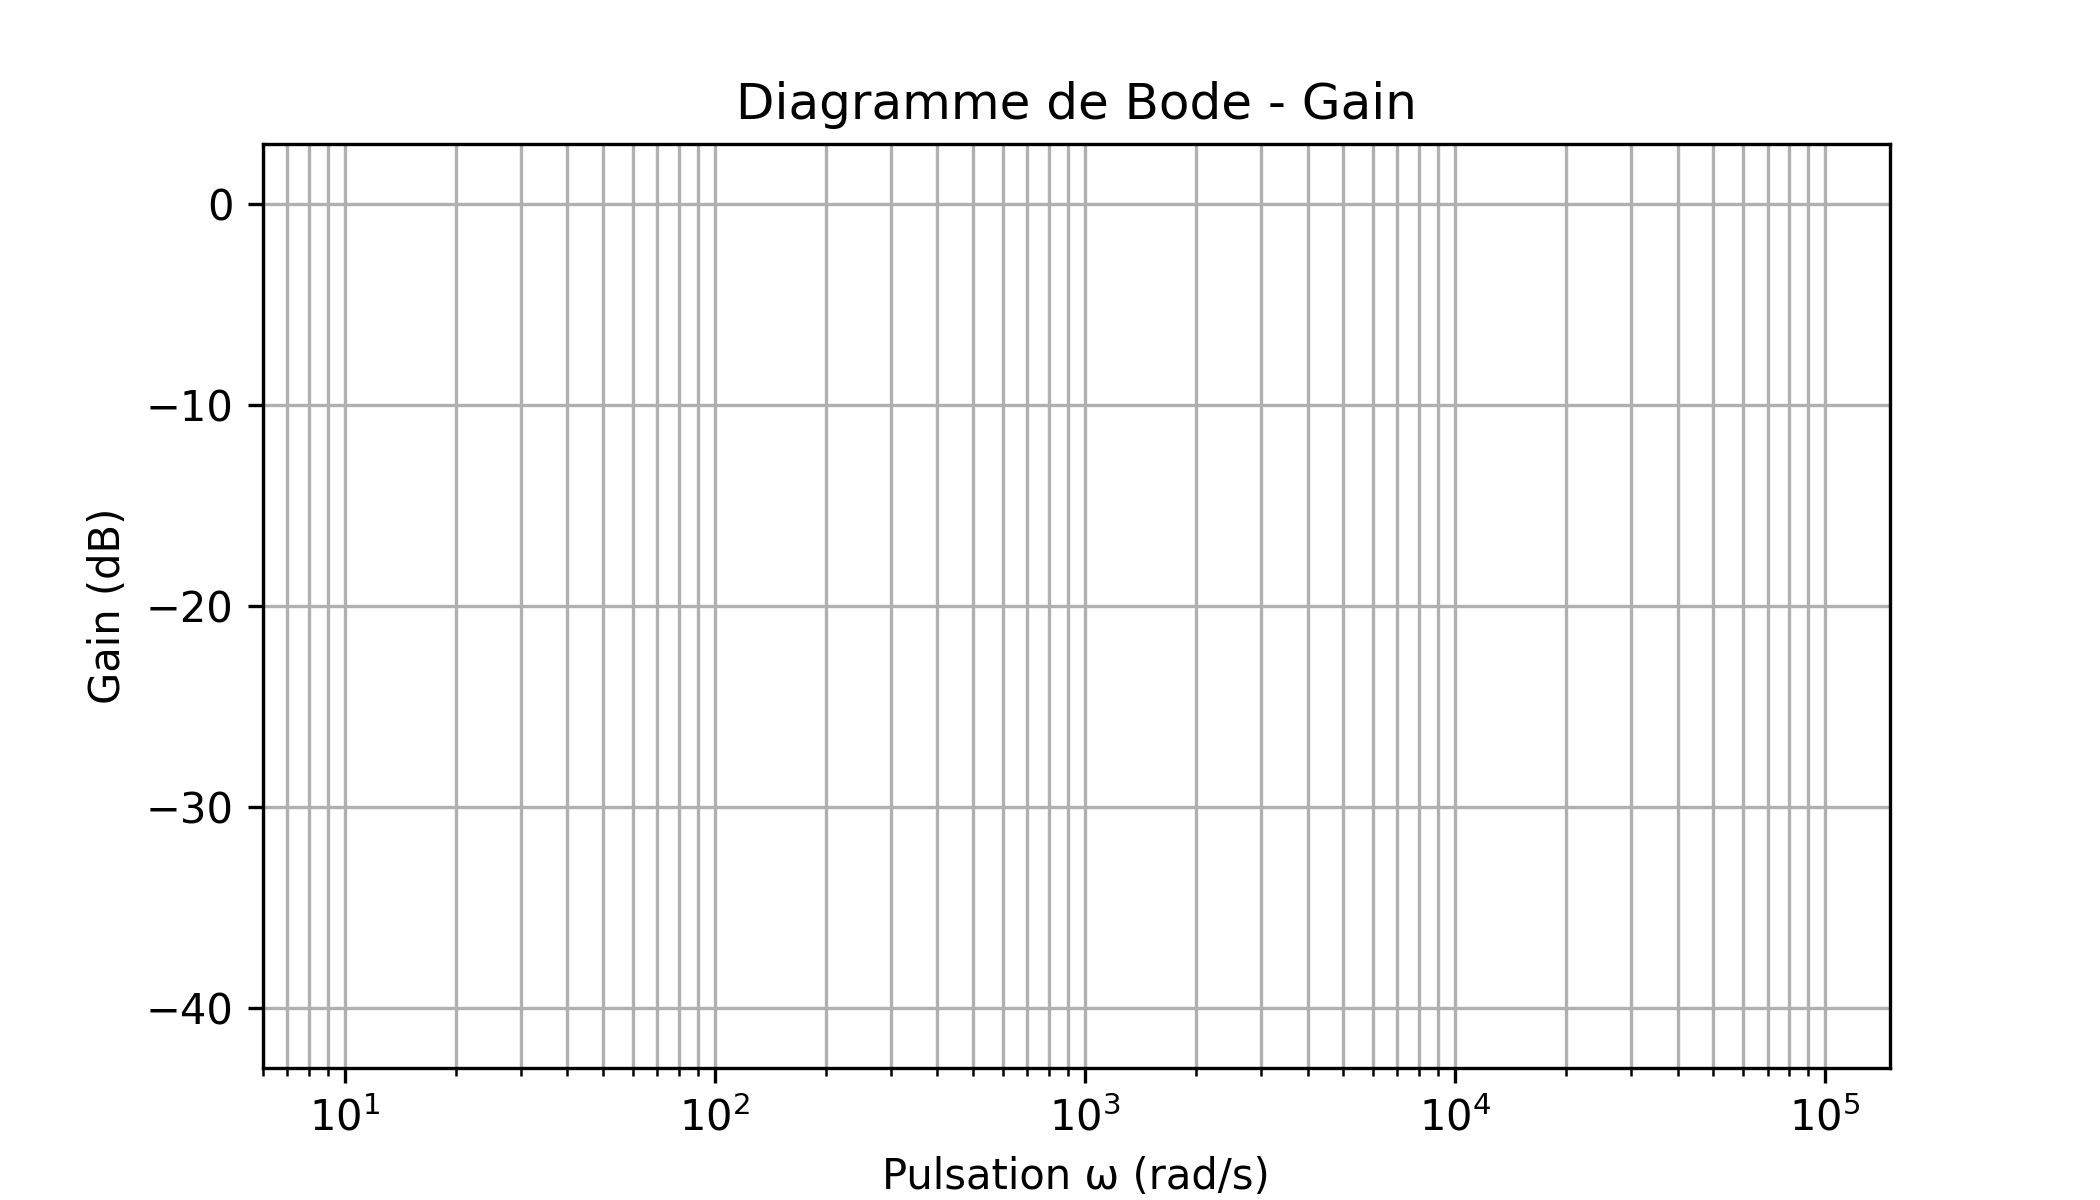
\includegraphics[width=1\linewidth]{bode diagrams/bode_gain.png}
        \end{subfigure}
        \hfill\begin{subfigure}{0.48\textwidth}
            \centering
            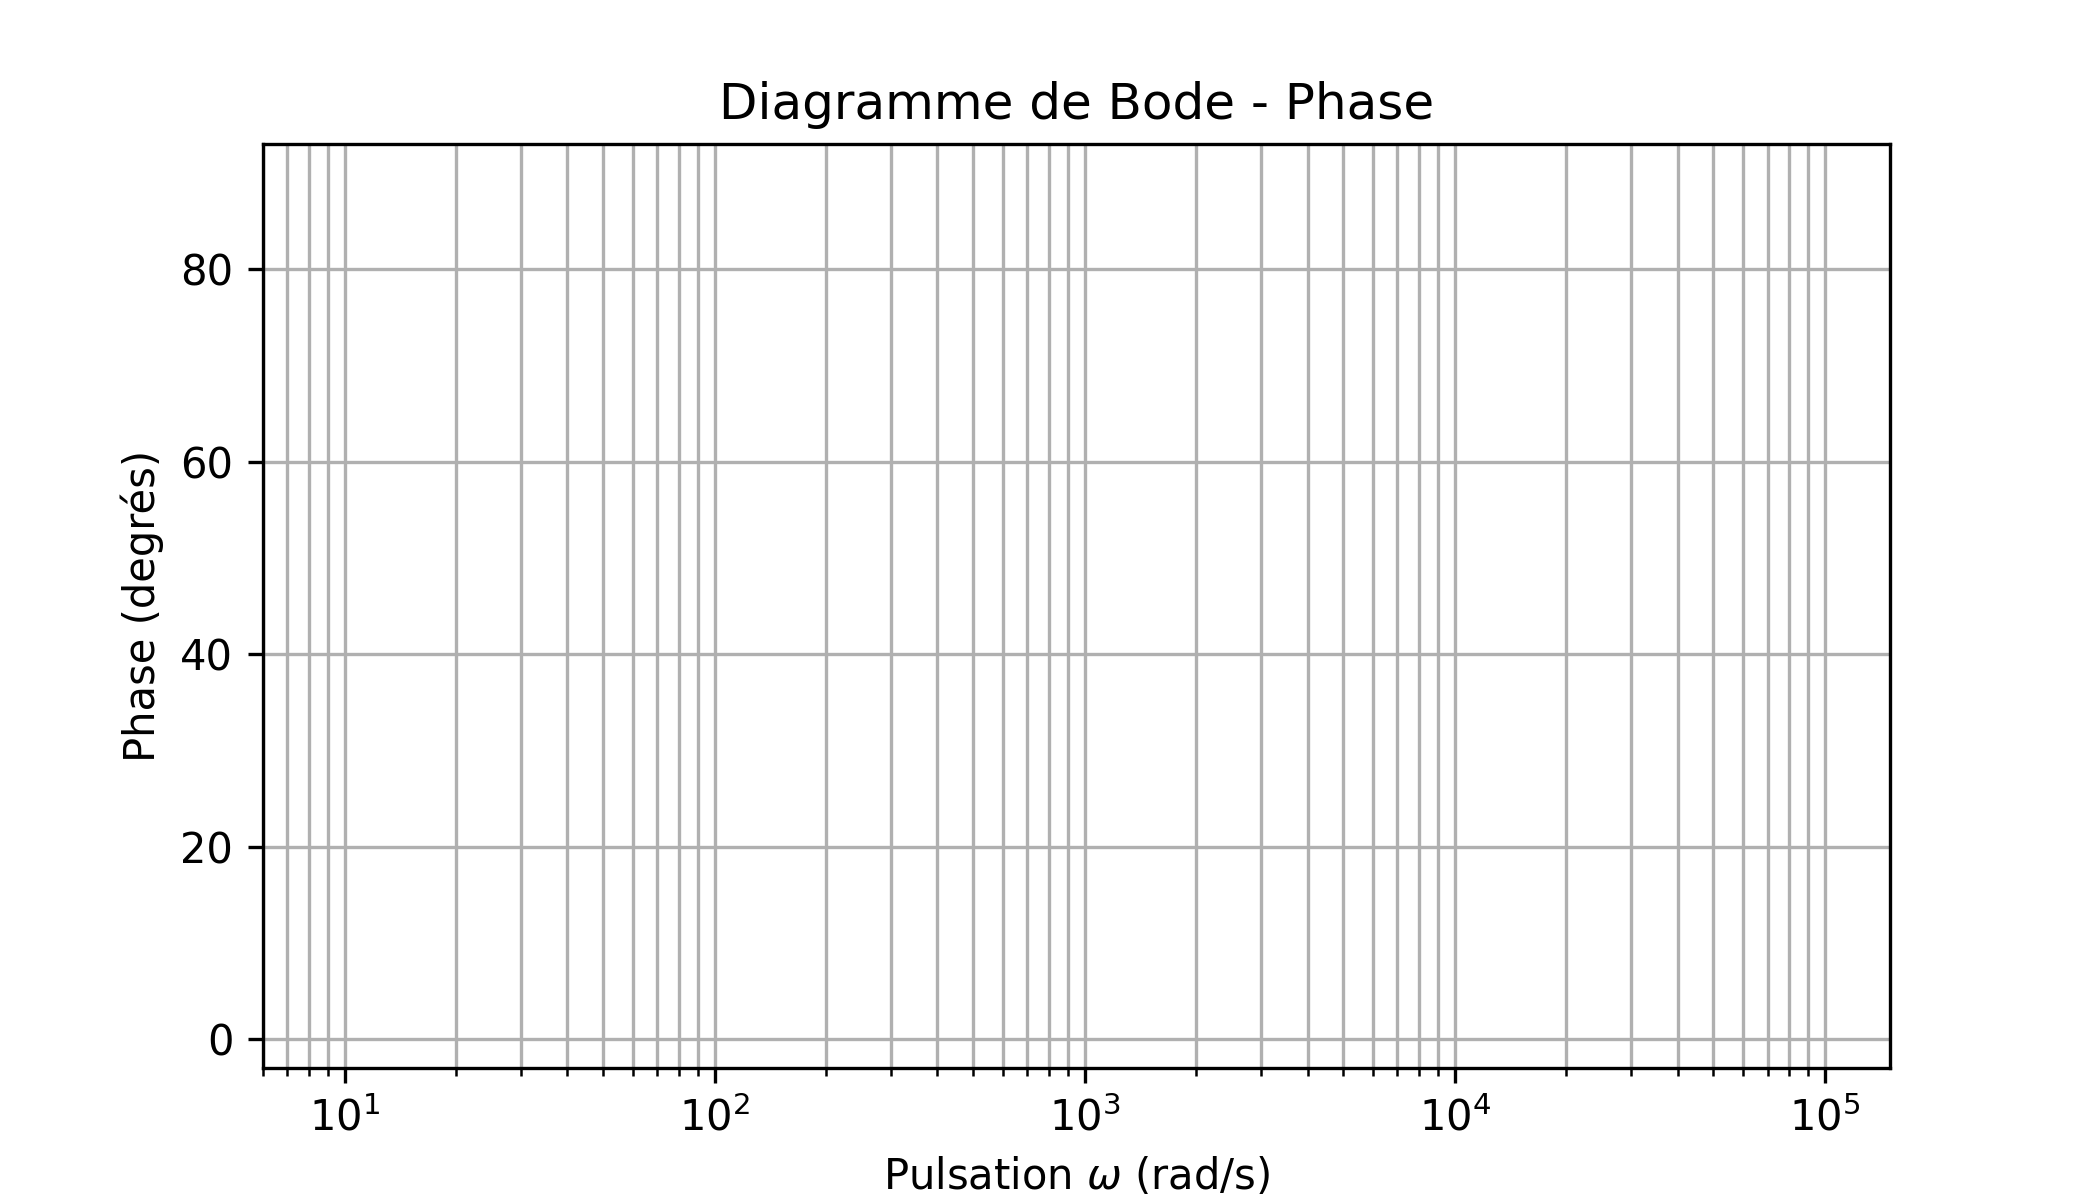
\includegraphics[width=1\linewidth]{bode diagrams/bode_phase.png}
        \end{subfigure}
    \end{figure}


    \section{Diviseur de Tension} \label{sec:Diviseur de Tension}
    \begin{wrapfigure}[4]{r}{0.5\textwidth}
        \centering
        \vspace{-1.5cm}
        \begin{circuitikz}        
            % Circuit code
            \draw (0,0) to[short,o-o] ++ (4,0);  % draw the bottom wire
            \draw (0,4) to[short,o-] ++ (2,0) coordinate(a);  
            \draw (a) to[R, name=Z1] ++ (0,-2) to[R, name=Z, *-*] ++ (0, -2);  % draw the two resistance
            \node at (Z1.center) {$\underline{Z}_1$};  % draw label "R" at the center of the resistance
            \node at (Z.center) {$\underline{Z}$};  % draw label "R" at the center of the resistance
            \draw (2,2) to[short, *-o] ++ (2,0);
            % Voltage labels
            \draw (0,4) to[open, v_=$V_{\text{in}}$\;] ++(0,-4);
            \draw (4,2) to[open, v^=\hspace{1.5mm} $V_{\text{out}}$] ++(0,-2);
        \end{circuitikz}
    \end{wrapfigure}

    \noindent La formule du pont diviseur de tension dans ce circuit est:
    $$V_{\text{out}} = V_{\text{in}} \times \dfrac{Z}{Z+Z_1}$$

    %La formule généralisée à $i$ résistances (notées $Z_i$) est:\\
    %$V_{\text{Z_r}} = V_{\text{in}} \times \dfrac{Z_r}{\sum_{i=1}^{n}Z_i}$
      
\clearpage

\vspace{2cm}
\section{Etude complète d'un filtre simple}

\begin{wrapfigure}[2]{r}{0.5\textwidth}
    \centering
    \vspace{-1.7cm}
    \begin{circuitikz}        
        % Circuit code
        \draw (0,0) to[short,o-o] ++ (4,0);  % draw the bottom wire
        \draw (0,2) to[R, name=R, o-] ++ (3,0) coordinate(a);  % draw the resistance
        \node at (R.center) {R};  % draw label "R" at the center of the resistance
        \draw (a) to[short,-o] ++ (1,0);  % draw wire to the right of R
        \draw (a) to[C, l_=C, *-*] ++(0,-2);  % draw the Capacitor

        % Voltage labels
        \draw (0,2) to[open,v_=V$_{\text{in}}$\;] ++(0,-2);
        \draw (4,2) to[open,v^=\hspace{1.5mm} V$_{\text{out}}$] ++(0,-2);
    \end{circuitikz}
\end{wrapfigure}


\subsection{Schéma électrique du filtre}
On reconnait un filtre passe-bas $RC$ du premier ordre.


\subsection{Comportement du filtre à basse et haute fréquence}

\begin{itemize}[label=$\ast$]
    \item $\omega \rightarrow 0$ : Le condensateur se comporte comme un interrupteur ouvert ($\underline{Z}_C \rightarrow +\infty$).\\
        $V_{\text{out}}=V_{\text{in}}$ \quad Le signal basse fréquence passe.
    \item $\omega \rightarrow +\infty$ : Le condensateur se comporte comme un fil ($\underline{Z}_C \rightarrow 0$).\\
        $V_{\text{out}} = 0$ \quad Le signal haute fréquence est coupé (car la tension au borne d'un fil est nulle).
\end{itemize}

\subsection{Calcul fonction de transfert}

$\underline{H}(j\omega) = \dfrac{\underline{u}_s}{\underline{u}_e} =  \dfrac{1}{\underline{u}_e}\times\underline{u}_e \times \dfrac{\dfrac{1}{jC\omega}}{\dfrac{1}{jC\omega} + R} = \dfrac{\dfrac{1}{jC\omega}}{\dfrac{1}{jC\omega} + R} = \dfrac{1}{1+jRC\omega} = \dfrac{1}{1+j\frac{\omega}{\omega_0}}$
\quad avec $\omega_0=\frac{1}{RC}$

$G = \left|\underline{H}(j\omega)\right| = \dfrac{1}{\sqrt{1+\left(\frac{\omega}{\omega_0}\right)^2}}$

$G_{dB} = 20\log{\left|\underline{H}(j\omega)\right|} $

\subsection{Etude asymptotique du gain}

\begin{itemize}[label=$\ast$]
    \item $\omega \rightarrow +\infty$ : $G_{dB} \rightarrow 20\log{\left(\dfrac{\omega_0}{\omega}\right)} = 20\log{(\omega_0)} - 20\log{(\omega)}$ \quad
    car $\frac{1}{\sqrt{1+\left(\frac{\omega}{\omega_0}\right)^2}} \underset{w \to \infty}{\sim} \frac{1}{\sqrt{\left(\frac{\omega}{\omega_0}\right)^2}} = \frac{\omega_0}{\omega} $\\
    La pente est alors de $-20\,dB$ par décade (multiplication/division par 10 de la pulsation) pour les hautes fréquences.
\end{itemize}


\begin{wrapfigure}[5]{r}{0.5\textwidth}
    \centering
    \vspace{-1cm}
    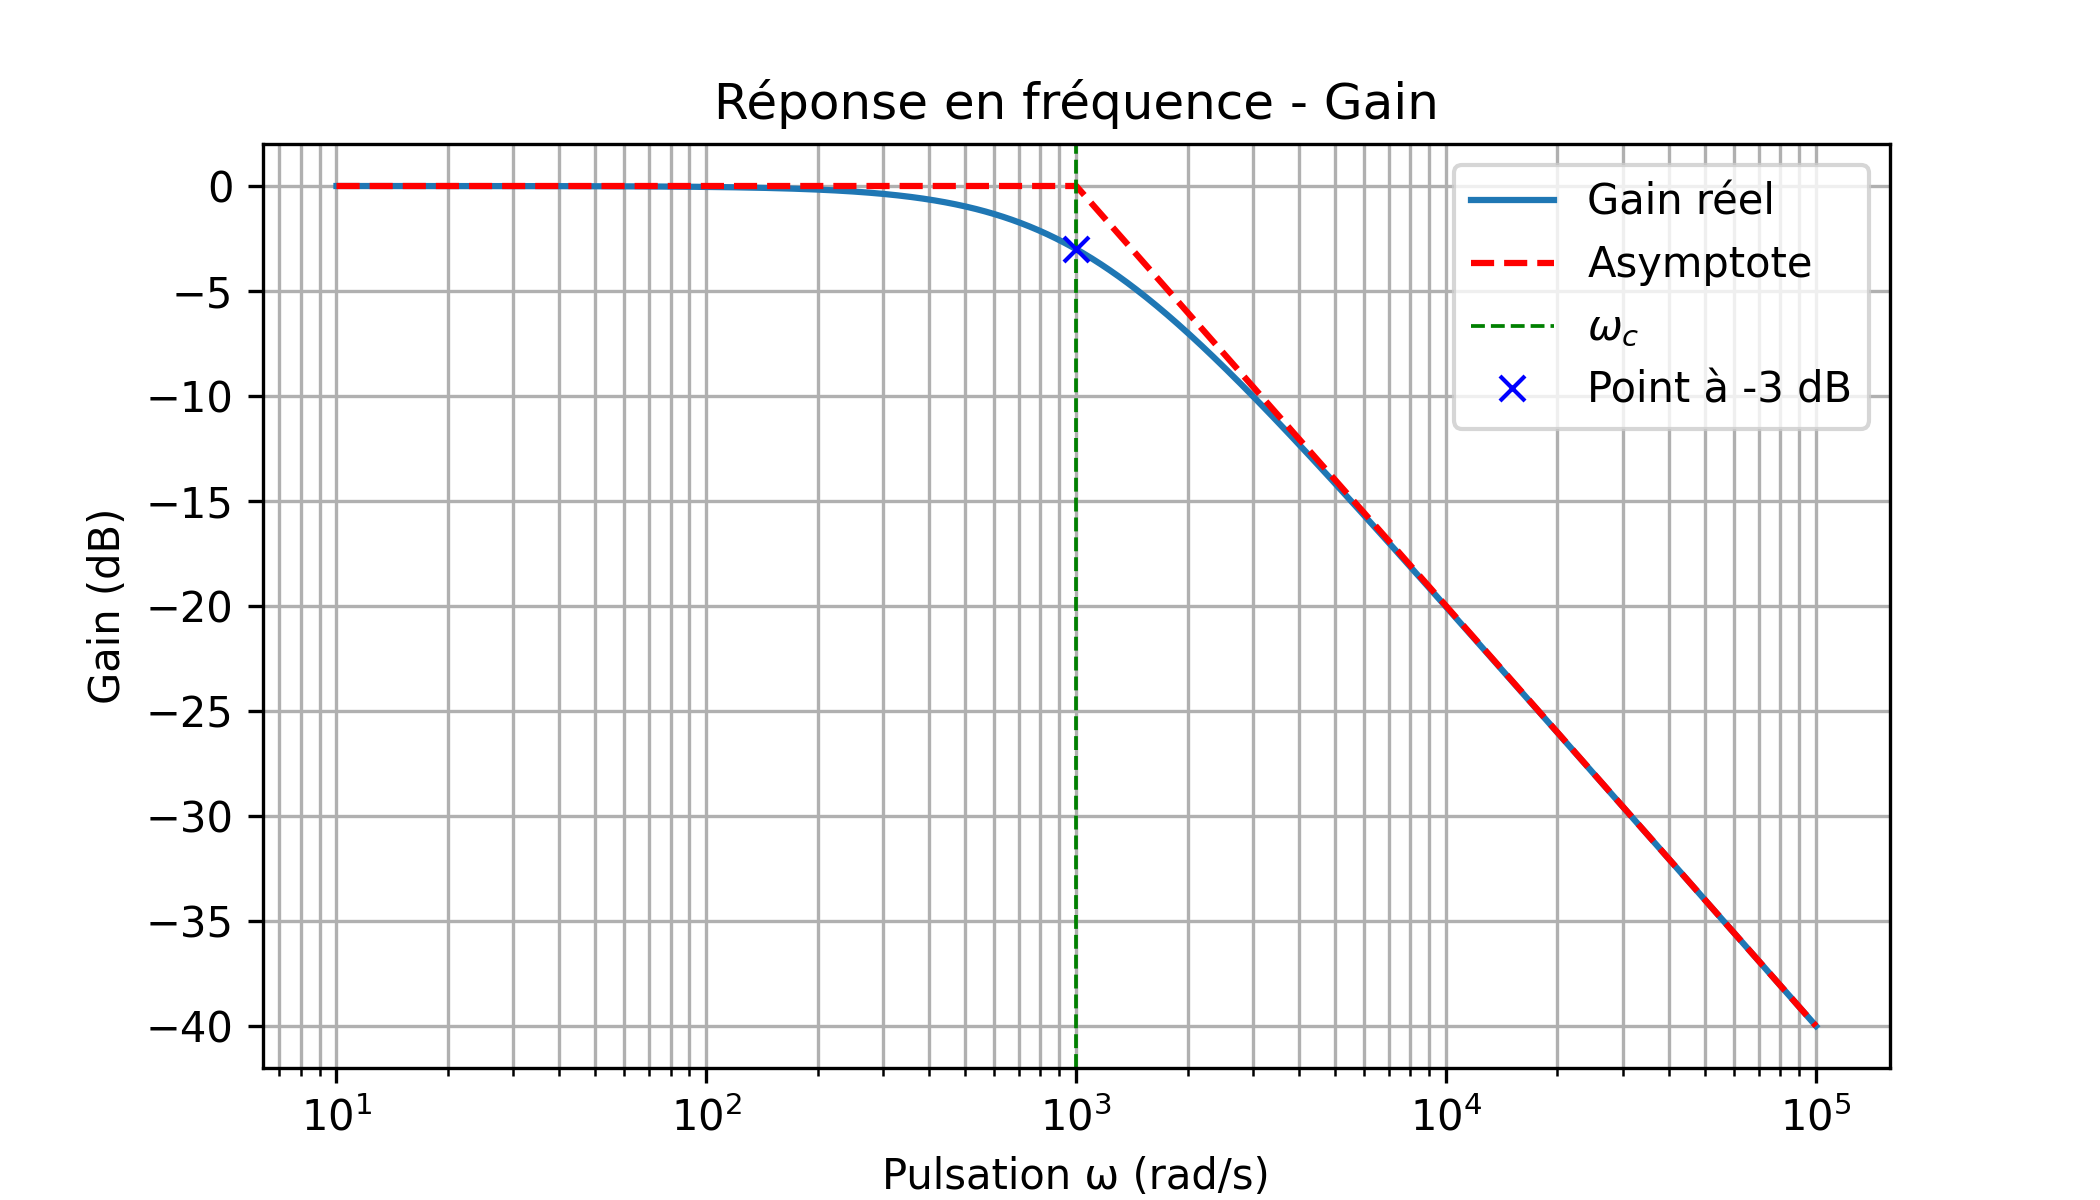
\includegraphics[width=0.6\textwidth]{bode diagrams/filtre_passe_bas_gain.png}
\end{wrapfigure}

    $\ast$ $\omega \rightarrow 0$ : $G_{dB} \rightarrow 1$\\
    \indent $\ast$ $\omega \rightarrow \omega_0$ : $G_{dB} \rightarrow 20\log{\left(\dfrac{1}{\sqrt{2}}\right)} \approx -3\,dB$

\vspace{3cm}

\subsection{Etude de la Phase}

\noindent On étudie la différence de phase entre le signal de sortie et le signal d'entré: $\varphi_{\underline{u}_s/\underline{u}_e}$\\
$\arg{(H)} = \arg{(1)}-\arctan{\left( \dfrac{\omega}{\omega_0} \right)} = -\arctan{\left( \dfrac{\omega}{\omega_0} \right)}$


\begin{wrapfigure}[5]{r}{0.5\textwidth}
    \centering
    \vspace{-1.5cm}
    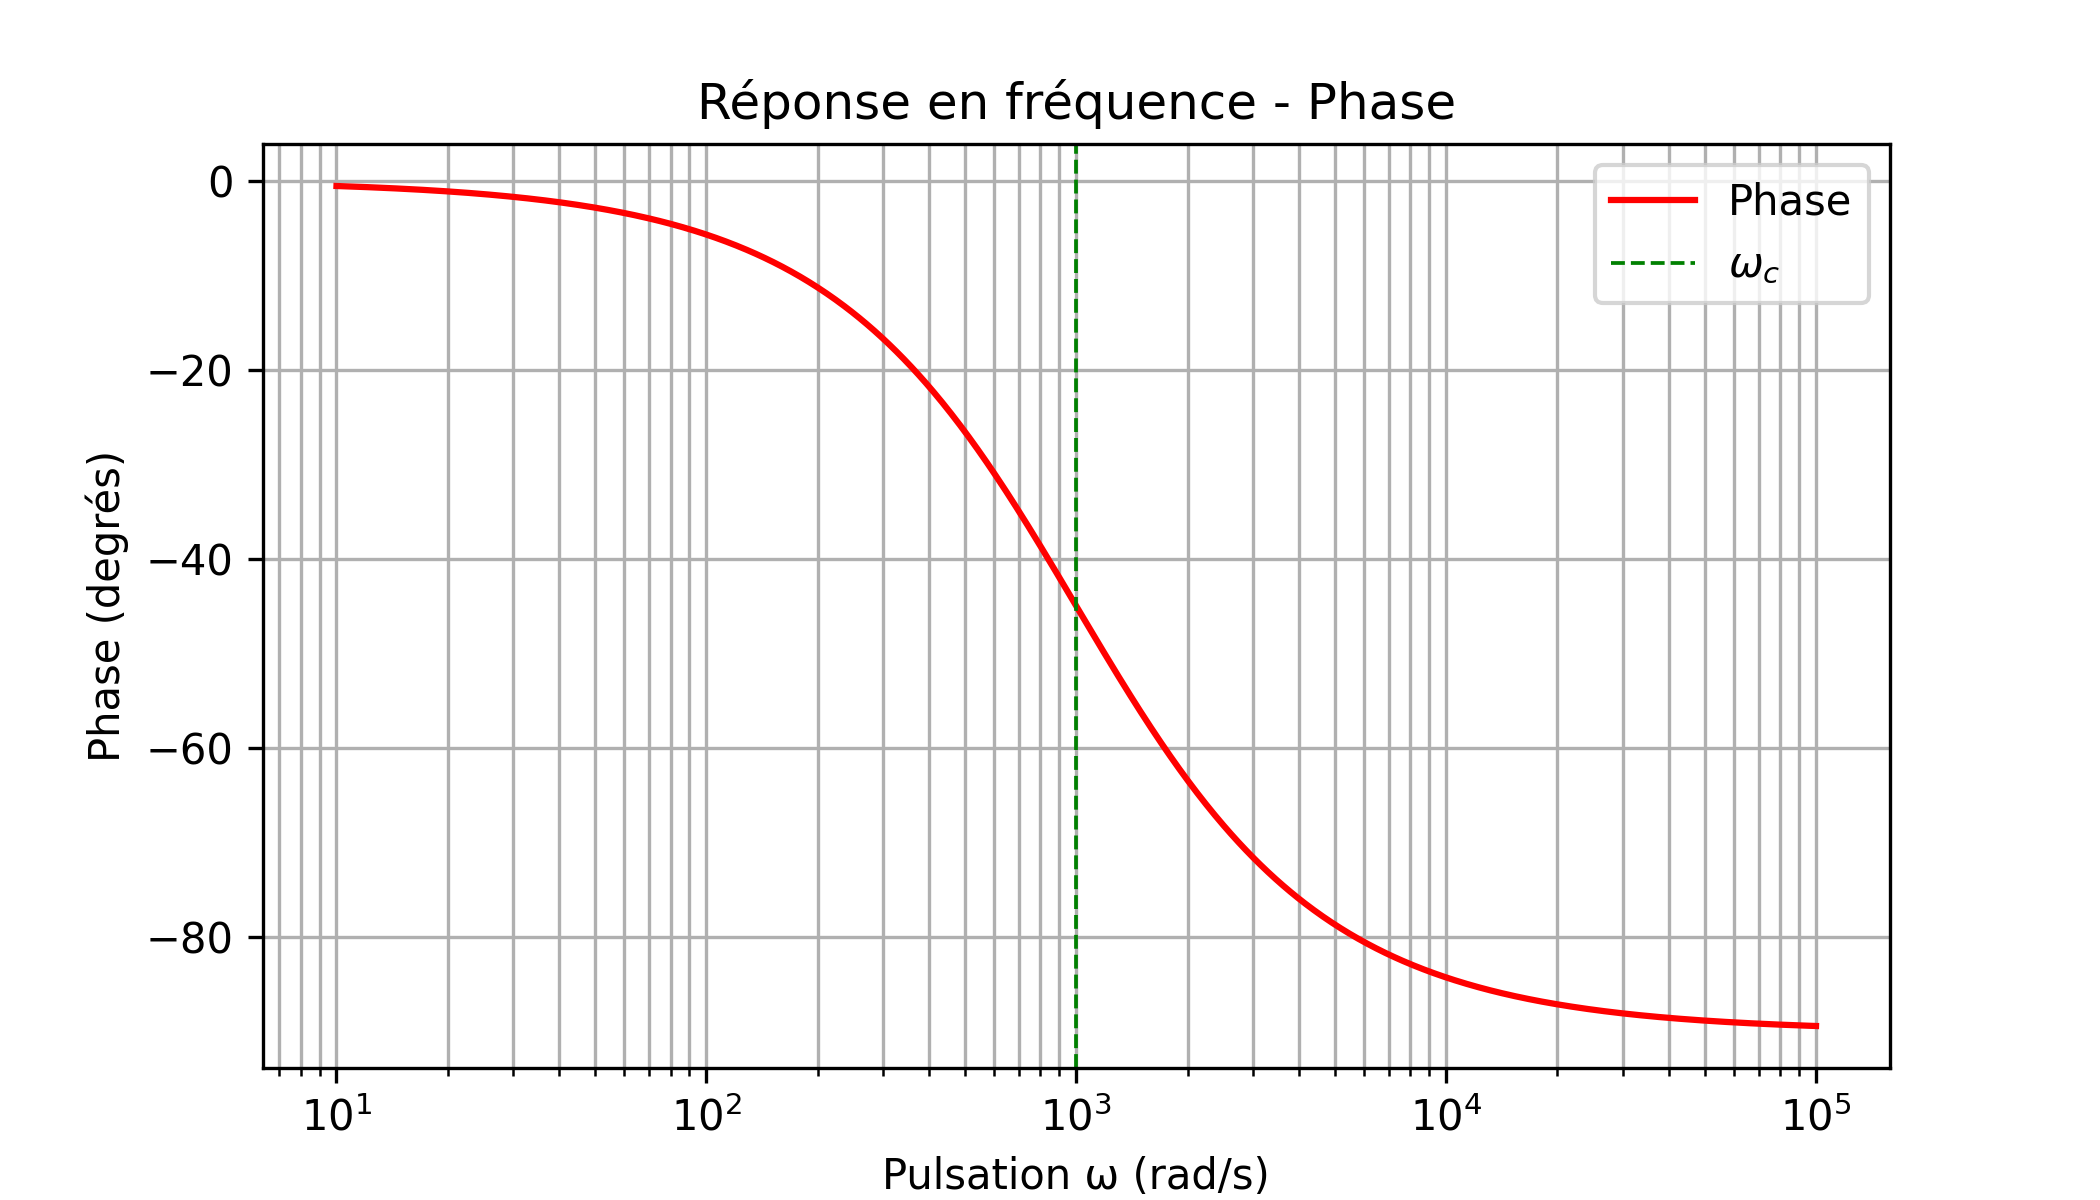
\includegraphics[width=0.5\textwidth]{bode diagrams/filtre_passe_bas_phase.png}
\end{wrapfigure}

    $\ast$ $\omega \rightarrow 0$ : $\arg{(H)} = -\arctan{(0)} \rightarrow 0$
\begin{itemize}[label=$\ast$]
    \item $\omega \rightarrow +\infty$ : $\arg{(H)} = -\arctan{\left( \dfrac{\infty}{\omega_0} \right)} \rightarrow -\dfrac{\pi}{2}$ 
    \item $\omega \rightarrow \omega_0$ : $\arg{(H)} = -\arctan{(1)} \rightarrow -\dfrac{\pi}{4}$
\end{itemize}

\clearpage

\section{Etude complète d'un filtre passe haut}

\subsection{Comportement du filtre à basse et haute fréquence}

\begin{wrapfigure}[5]{r}{0.5\textwidth}
    \centering
    \vspace{-0.5cm}
    \begin{circuitikz}        
        % Circuit code
        \draw (0,0) to[short,o-o] ++ (4,0);  % draw the bottom wire
        \draw (0,2) to[R, name=R, o-] ++ (3,0) coordinate(a);  % draw the resistance
        \node at (R.center) {R};  % draw label "R" at the center of the resistance
        \draw (a) to[short,-o] ++ (1,0);  % draw wire to the right of R
        \draw (a) to[L, l_=L, *-*] ++(0,-2);  % draw the Capacitor

        % Voltage labels
        \draw (0,2) to[open,v_=V$_{\text{in}}$\;] ++(0,-2);
        \draw (4,2) to[open,v^=\hspace{1.5mm} V$_{\text{out}}$] ++(0,-2);
    \end{circuitikz}
\end{wrapfigure}



    $\ast$  $\omega \rightarrow 0$ : La bobine se comporte comme un fil ($\underline{Z}_L \rightarrow 0$).\\
        $V_{\text{out}}=0$ \quad Le signal basse fréquence est coupé.

    $\ast$  $\omega \rightarrow +\infty$ : La bobine se comporte comme un interrupteur ouvert ($\underline{Z}_L \rightarrow +\infty$).\\
        $V_{\text{out}} = V_{\text{in}}$ \quad Le signal haute fréquence passe.

\subsection{Calcul fonction de transfert}

$\underline{H}(j\omega) = \dfrac{\underline{u}_s}{\underline{u}_e} = \dfrac{jL\omega}{jL\omega + R} = \dfrac{\dfrac{jL\omega}{R}}{1 + \dfrac{jL\omega}{R}} = \dfrac{\dfrac{j\omega}{\omega_0}}{1 + \dfrac{j\omega}{\omega_0}}$
\quad avec $\omega_0=\frac{R}{L}$

On pourrait décomposer la fonction de transfert afin de retrouver la fonction de transfert d'un filtre passe bas. \quad
$\underline{H}(j\omega) = \underline{H}_1(j\omega) * \underline{H}_2(j\omega) = \dfrac{j\omega}{\omega_0} * \dfrac{1}{1 + \dfrac{j\omega}{\omega_0}} $

$G_{dB} = 20\log{\left|\underline{H}(j\omega)\right|} =  20\log{\left( \dfrac{\frac{\omega}{\omega_0}}{\sqrt{1+(\frac{\omega}{\omega_0})^2}} \right)}$

\subsection{Etude asymptotique du gain}

\begin{wrapfigure}[5]{r}{0.5\textwidth}
    \centering
    \vspace{-2.5cm}
    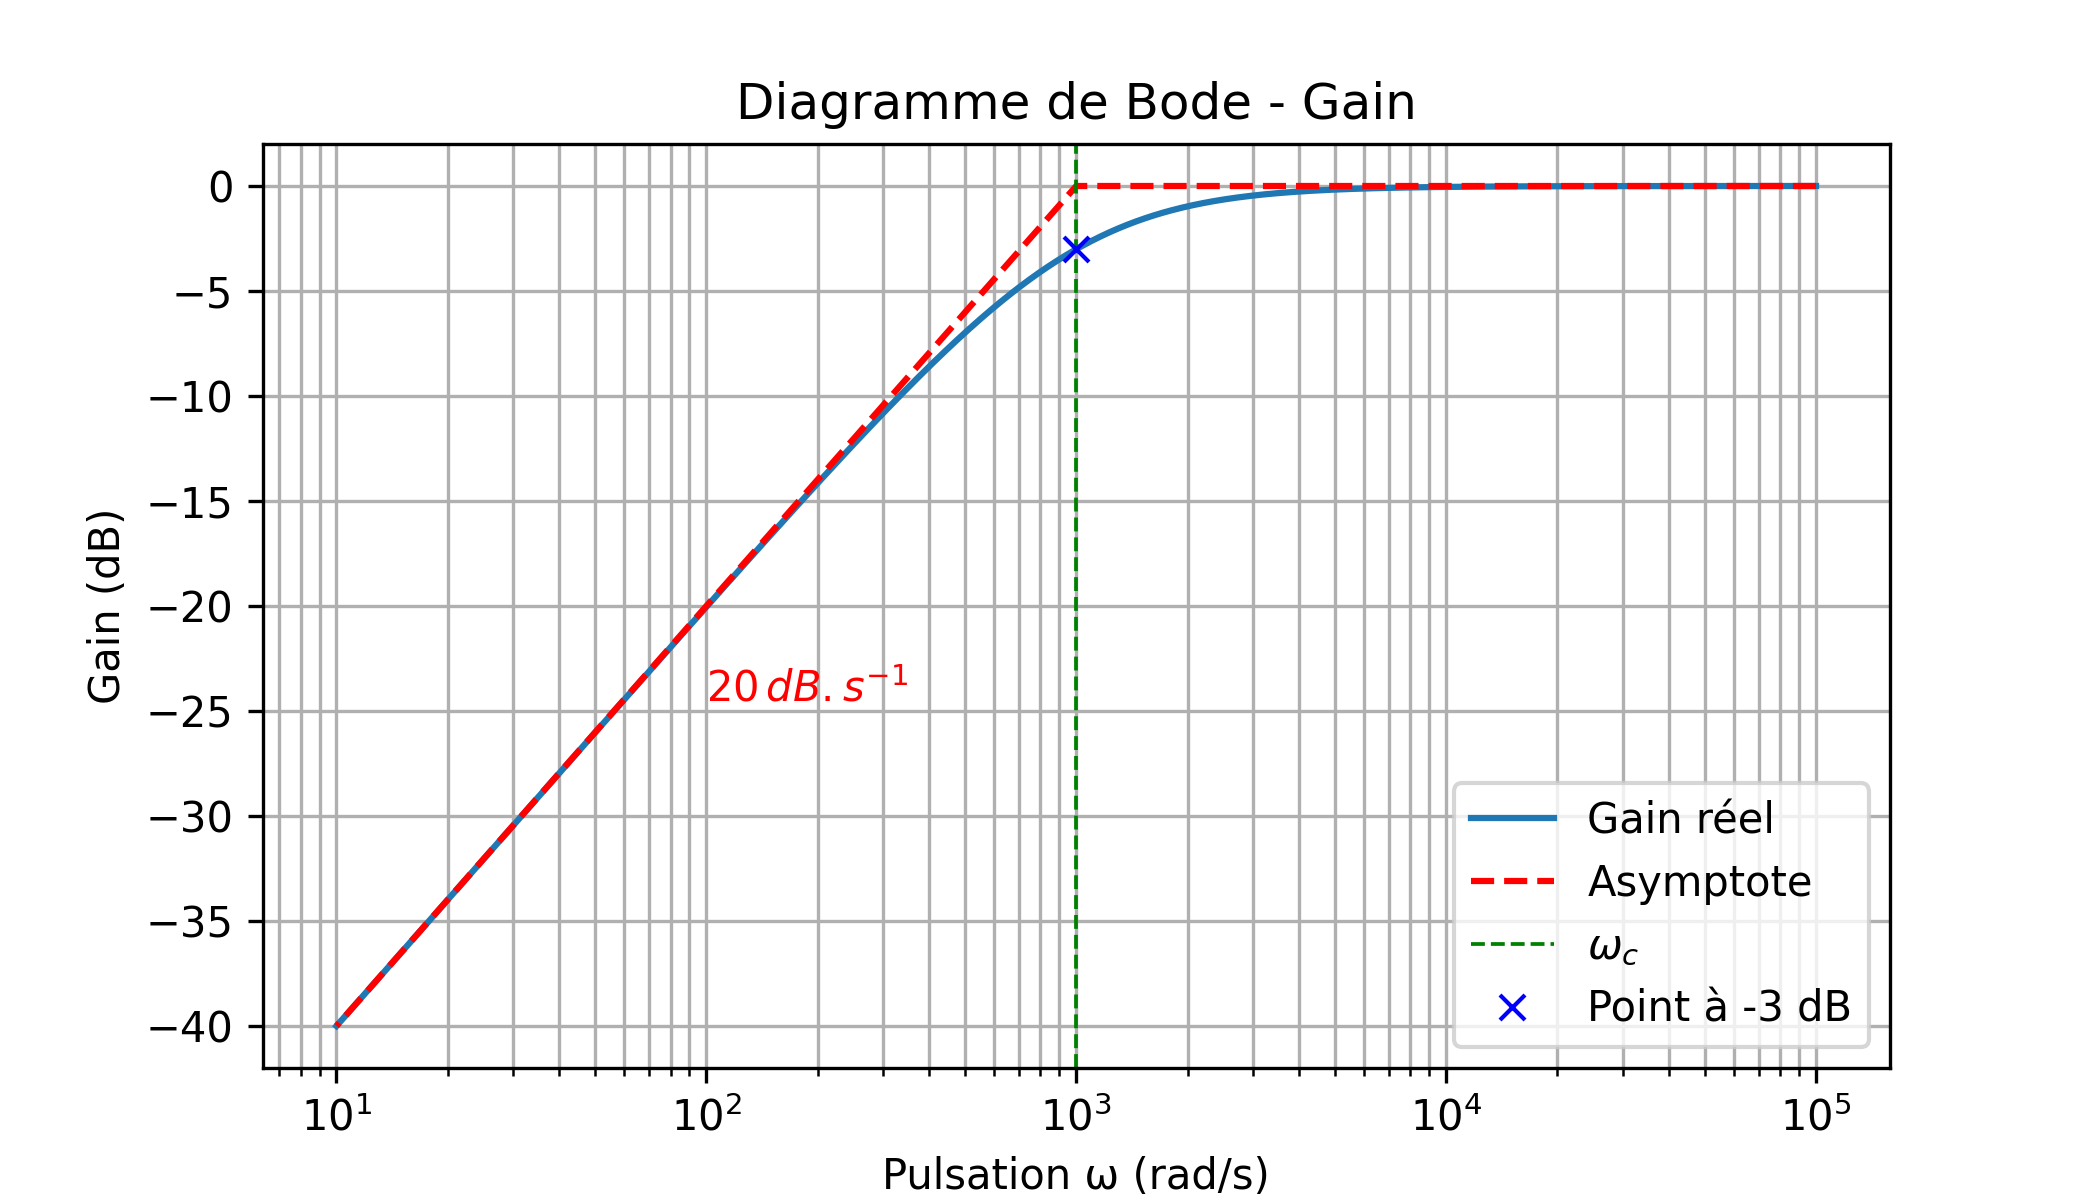
\includegraphics[width=0.6\textwidth]{bode diagrams/filtre_passe_haut_gain.png}
\end{wrapfigure}

    $\ast$ $\omega \rightarrow 0$ : $G_{dB} \rightarrow 20\log{\left( \dfrac{\omega}{\omega_0} \right)}$\\
    \indent $ = 20\log{(\omega)} - 20\log{(\omega_0)} \rightarrow -\infty$\\
    \indent La pente est alors de $+20\,dB$ par décade.
\begin{itemize}[label=$\ast$]
        \item $\omega \rightarrow +\infty$ : $G_{dB} \rightarrow 20\log{(1)} = 0$
    \item $\omega \rightarrow \omega_0$ : $G_{dB} \rightarrow 20\log{\left(\dfrac{1}{\sqrt{2}}\right)} \approx -3\,dB$
\end{itemize}   


\subsection{Etude de la Phase}

\noindent On étudie la différence de phase entre le signal de sortie et le signal d'entré: $\varphi_{\underline{u}_s/\underline{u}_e}$\\
$\arg{(H)} = \arg{(1)}-\arctan{\left( \dfrac{\omega}{\omega_0} \right)} = -\arctan{\left( \dfrac{\omega}{\omega_0} \right)}$

\begin{wrapfigure}[5]{r}{0.5\textwidth}
    \centering
    \vspace{-1cm}
    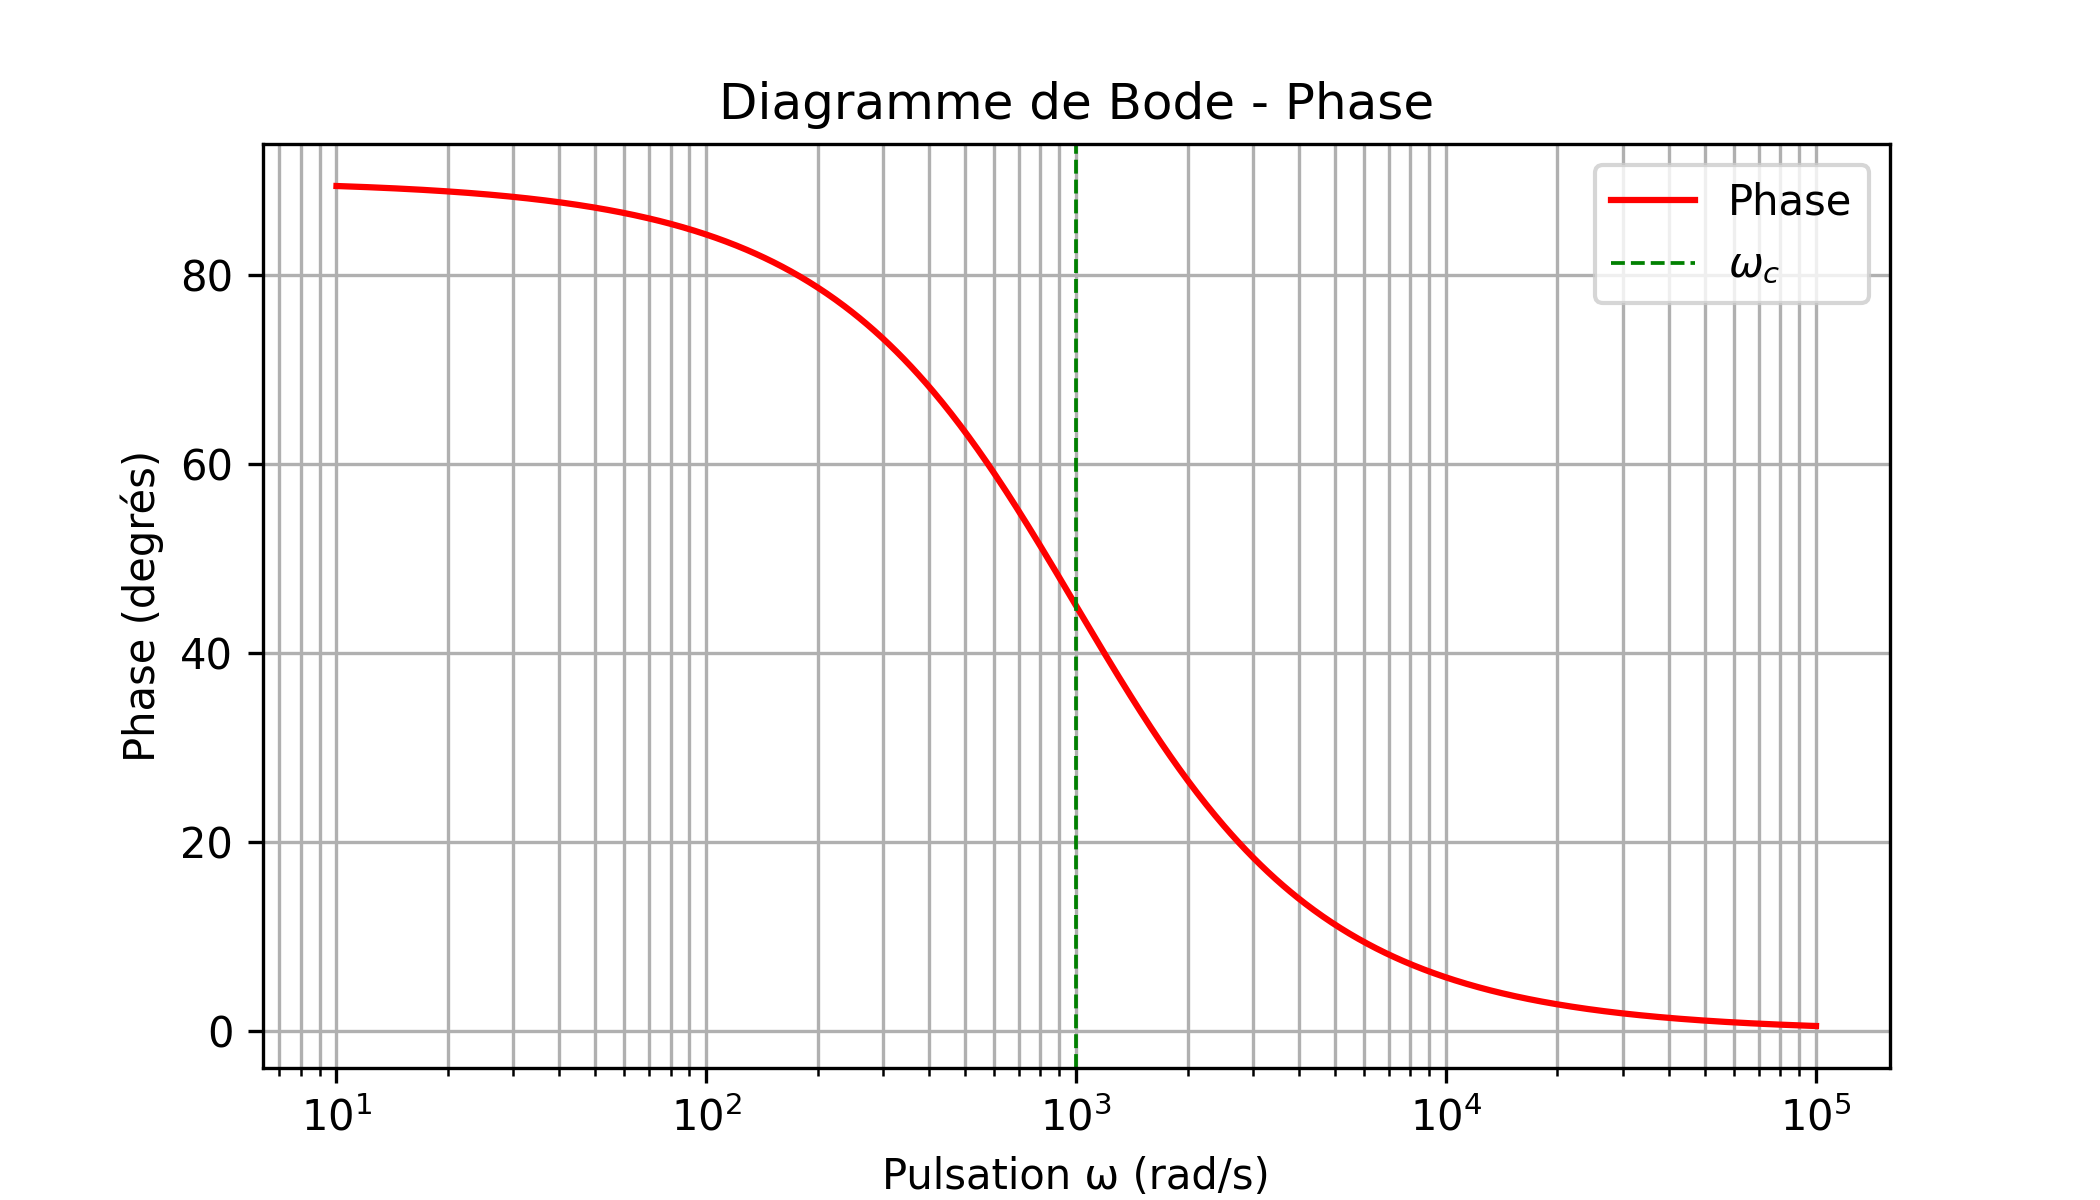
\includegraphics[width=0.6\textwidth]{bode diagrams/filtre_passe_haut_phase.png}
\end{wrapfigure}

    $\ast$ $\omega \rightarrow 0$ : $\arg{(H)} = -\arctan{(0)} \rightarrow 0$
\begin{itemize}[label=$\ast$]
    \item $\omega \rightarrow +\infty$ : $\arg{(H)} = -\arctan{\left( \dfrac{\infty}{\omega_0} \right)} \rightarrow \dfrac{\pi}{2}$ 
    \item $\omega \rightarrow \omega_0$ : $\arg{(H)} = -\arctan{(1)} \rightarrow \dfrac{\pi}{4}$
\end{itemize}


\end{document}